\documentclass{adonis}
\usepackage{hyperref}
\usepackage{tabularx}
\usepackage{xurl}
\usepackage{minted}
\usepackage{graphicx}
\usepackage{fontawesome}
\usepackage[export]{adjustbox}


% main details
\title{Generate Answer to Visual Questions in the Medical Domain: Phase 2}
\author{Niki Nezakati - 98522094
\\
\href{https://github.com/nikinezakati/medical-gen-vqa/tree/phase-two}{\faicon{github}} GitHub Repository}




\begin{document}
\definecolor{bg}{rgb}{0.66,0.66,0.66}
	\maketitle
	\section{Creating the Full Sentence Dataset}
	
       In this research, I conducted a study that involved the utilization of the SLAKE \cite{slake} dataset, as discussed in phase one. The objective was to generate comprehensive answers from both single and multi-word answers present in the dataset. To accomplish this, I employed the proposed method outlined in the FSVQA \cite{FSVQA} article. In order to convert the answers into complete sentences, I leveraged the NLTK language tool and pattern.en part-of-speech tagger. Taking into consideration the relevant question and answer, we applied the language rules introduced in the FSVQA article. A detailed description of these language rules can be found in the table \ref{table1} from this article. By implementing these rules on the SLAKE dataset, we successfully obtained a new dataset comprising answers in the form of complete sentences.
       

       \begin{table}[h]
        \center{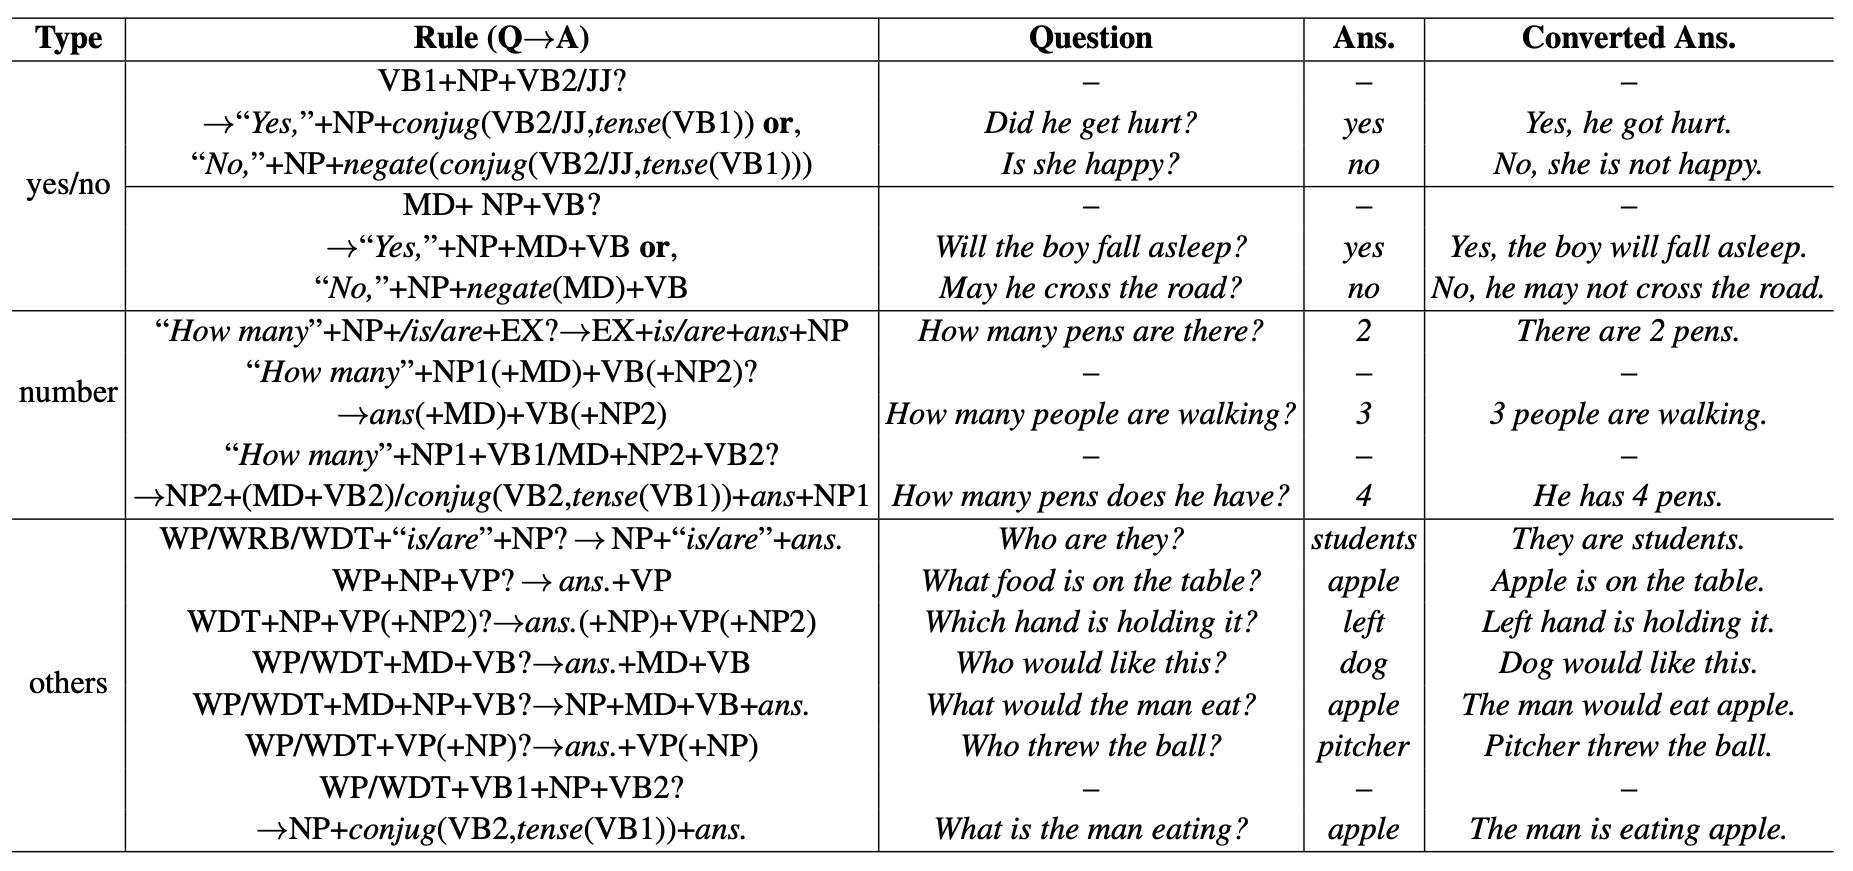
\includegraphics[width=1\textwidth]{images/language-rules.png}}
        \caption{General conversion rules for converting captions to questions.}
    \label{table1}
        % \vspace{-2mm}    
\end{table}

To do this, you should run the bash script located in the run folder named generate\_fs\_answers.sh. You can add one argument to this bash which is the output directory and you can specify that or leave it as the default value (data/full\_sentence\_data).

        \begin{minted}[bgcolor=bg]{python}
        bash run/generate_fs_answers.sh
        \end{minted}

        
  After executing the provided bash script, you will have access to the resulting dataset.  This dataset contains medical images along with corresponding question and full-sentence answer. 


\section{Word2Vec}
	
        In order to train Word2Vec on different data categories including Color, KG, Modality, Organ, Plane, Position, Shape, and Size, you should run the bash script located in the run folder named train\_word2vec.sh. You should add the category names and number of iterations to this bash. 
        \begin{minted}[bgcolor=bg]{python}
        bash run/dataset_tokenization.sh
        \end{minted}

		
		\section{Tokenization}

        Accurately processing questions entails breaking them down into smaller parts or tokens to enable deep neural networks to carry out the necessary computations. In the context of our experiments, where both the LXMERT and VisualBERT networks are utilized, we rely on BERT network tokenization to extract the features of the input text. This choice is made because both LXMERT and VisualBERT models are built upon the BERT network.
	
        To do this, you should run the bash script located in the run folder named dataset\_tokenization.sh. You should add the annotations and questions paths to this bash, in addition to the tokenizer set to [lxmert]. The output result would be saved in (data/train/tokenized), (data/val/tokenized), and (data/test/tokenized).
        \begin{minted}[bgcolor=bg]{python}
        bash run/dataset_tokenization.sh
        \end{minted}


        \section{Image Feature Extraction}

        In this study, we employed 4096-dimensional features extracted from the second fully connected layer (fc7) of the VGG model, which consists of 19 layers and was pre-trained on the ImageNet dataset, as our image features. The images were inputted into this model, with each image being treated as having 36 bounding boxes. Subsequently, each bounding box was mapped to a 1024-dimensional feature vector.
	
        To do this, first we should resize the images. For this run the bash script located in the run folder named resize\_images.sh. Afterwards, you should run the bash script located in the run folder named extract\_image\_features.sh. You can add one argument to this bash which is the output directory and you can specify that or leave it as the default value (data/imgs).
        \begin{minted}[bgcolor=bg]{python}
        bash run/resize_images.sh
        bash run/extract_image_features.sh
        \end{minted}

    



 \section{Language Model and Model Architecture}
 In this research, inspired by the work of "Generate Answer to Visual Questions with Pre-trained Vision-and-Language Embeddings" \cite{genvqa} we examine 4 model architectures. We utilise VisualBERT and LXMERT embedding space with two different generative decoder heads, including Attention RNNs and Transformers. In order to determine the most effective architecture for visual question answering in the medical domain, we conduct a comprehensive evaluation that combines qualitative and quantitative analysis along with a Human Error Analysis.  We use BLEU, METEOR, and RougeL as our n-gram-based metrics, in addition to Average score and BERTScore as our embedding-based metrics.

 
To do this, you should run the bash script located in the run folder named train\_genVQA.sh. You should add the encoder type, decoder type, rnn type, number of rnn layers, the bidirectionallity of the rnn, attention type, attention method, and number of heads and layers if you are utilizing the transformer decoder. The output result containg the scores would be saved in logs directory, named as the time and date of run.


\begin{minted}[bgcolor=bg]{python}
        bash run/train_genVQA.sh
\end{minted}

The table below shows the performance of the different models.

    \begin{table}[h]
        \centering
        \resizebox{\textwidth}{!}{
        \begin{tabular}{llccccccc}
            \hline
            \multicolumn{2}{l}{Method} &  & \multicolumn{3}{c}{Word-based} &  & \multicolumn{2}{c}{Embedding-based}\\ 
            \cline{0-1} \cline{4-6} \cline{8-9}
            Encoder & Encoder & & BLEU & METEOR & ROUGE-L& & \lr{Average Score} & \lr{BERT Score} \\
            \hline
            \multirow{2}{*}{VisualBERT} 
            
             & \lr{1-LSTM+Bahdanau attention} & & \textbf{\underline{\lr{61.20}}} & \textbf{\underline{\lr{81.81}}} & \textbf{\underline{\lr{79.06}}} & & \textbf{\underline{\lr{96.33}}} & \textbf{\underline{\lr{89.05}}} \\
            
             & \lr{3-Transformer} & & \lr{12.30} & \lr{14.11} & \lr{15.00} &  & \lr{61.89} & \lr{33.89} \\
            \hline
            
            \multirow{2}{*}{LXMERT} 
             & \lr{1-LSTM+Bahdanau attention} & & \lr{56.78} & \lr{77.25} & \lr{75.37} &  & \lr{95.10} & \lr{85.36}\\
             
            & \lr{3-Transformer Decoder} & & \lr{24.94} & \lr{52.26} & \lr{53.89} &  & \lr{70.59} & \lr{69.10} \\
            \hline
        \end{tabular}
        
        }
        \caption{Results of our proposed models on the created dataset. The numbers in the decoder names mean the number of layers}
        \label{table2}
        % \vspace{-2mm}    
    \end{table}


As we can see by the results, The utilization of the LSTM recurrent neural network in combination with the attention mechanism as a decoder exhibits superior performance compared to Transformers. One contributing factor to this observation is the limited size of the dataset. Transformers often struggle when confronted with small datasets due to their extensive parameterization and high model capacity. These models, known for their data-hungry nature, require substantial training data to effectively capture complex patterns and generalize to unseen examples. In scenarios with small datasets and a constrained number of training samples, Transformers may lack the necessary diversity and coverage of underlying patterns, consequently leading to overfitting. Furthermore, the large number of parameters in Transformers exacerbates this issue by allowing the models to memorize the limited training samples, hampering their ability to generalize to new data.

Additionally, the quadratic computational complexity introduced by the self-attention mechanism in Transformers becomes particularly challenging to manage when working with smaller datasets. Consequently, the combination of data scarcity and computational inefficiency hampers Transformers' ability to learn meaningful representations from limited data. On the other hand, LSTM, along with attention, excels in capturing sequential dependencies and exhibits more effective handling of inputs with variable length. The recurrent nature of LSTM enables it to retain context from previous time steps, facilitating the modeling of temporal dependencies within the data. Furthermore, the attention mechanism selectively focuses on relevant parts of the input sequence, allowing the model to concentrate on crucial information. In contrast, Transformers operate in parallel and lack frequent connections, making them less suitable for tasks involving sequential data.

The improved performance of LSTM in conjunction with careful attention can be attributed to its robust architecture for capturing temporal patterns, which translates into enhanced performance in various tasks such as translation, text generation, and, in the context of this research, generating answers for image-related questions.

\section{Human Analysis}

In addition to the standard measurement criteria, this research incorporates a human evaluation process to assess the performance of the visual question answering system. For this purpose, a subset of elements was randomly selected from the dataset and subjected to evaluation using the superior model that was trained with the described architecture. Human evaluators carefully examined the answers generated by the system and categorized them into four distinct categories based on the type of mistakes observed: 

\begin{itemize}
    \item \textbf{EM} (Exact Match)
    \item \textbf{WA} (Wrong Answer): The model only generates incorrect VQA single/multi-word answers while the context and description are correct.
    \item \textbf{GE} (Grammatical Error)
    \item \textbf{WD} (Wrong Description): The model generates the correct VQA single/multi-word answer, but the description is wrong.
\end{itemize}

The table below illustrates some of these errors.

\vspace{3pt}

 \begin{center}
       \hspace*{-0.2cm}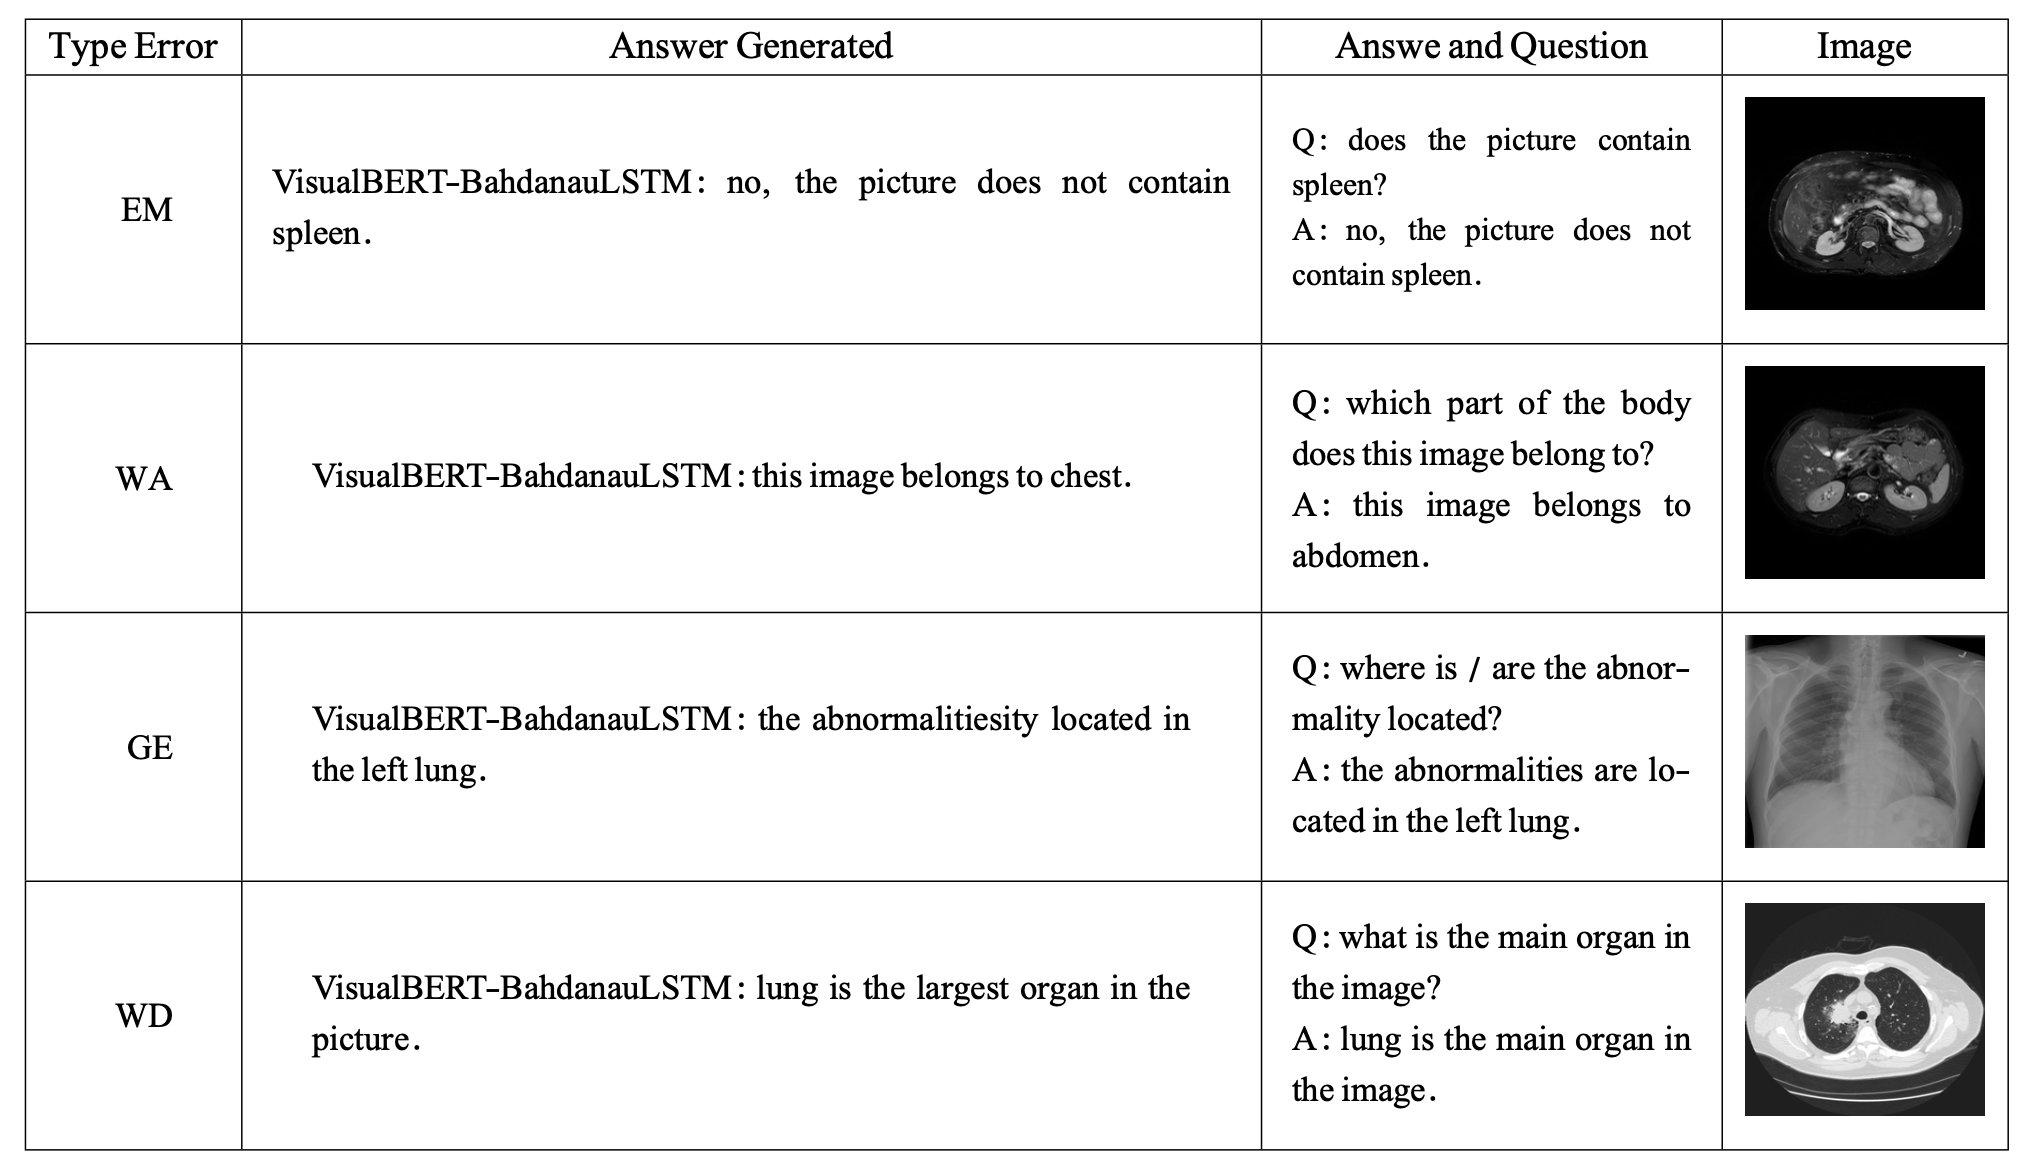
\includegraphics[width=12.5cm]{images/eval_table.png}
\end{center}




%   \begin{table}[H]
%   \centering
%   \setlength{\tabcolsep}{0.5em}
%   {\renewcommand{\arraystretch}{1.2}
%     \begin{minipage}{15.5cm}
%   \begin{tabular}{ | l | c | r | }
%     \hline
%     Uncom. Uniq. Train Ans. & Uncom. Uniq. Valid Ans. & Uncom. Uniq. Test Ans. \\ \hline
%     45 & 54 & 50 \\ \hline
% \end{tabular}
%   \end{minipage}}
%   \end{table}

  
% \newpage
% \vspace{10pt}
%   Finally, the histograms displayed below represent the frequency of occurrence for the top 20 most unique label tokens, considering the large number of distinct tokens involved in the answers.
  
%  \begin{center}
%        \hspace*{-1.5cm}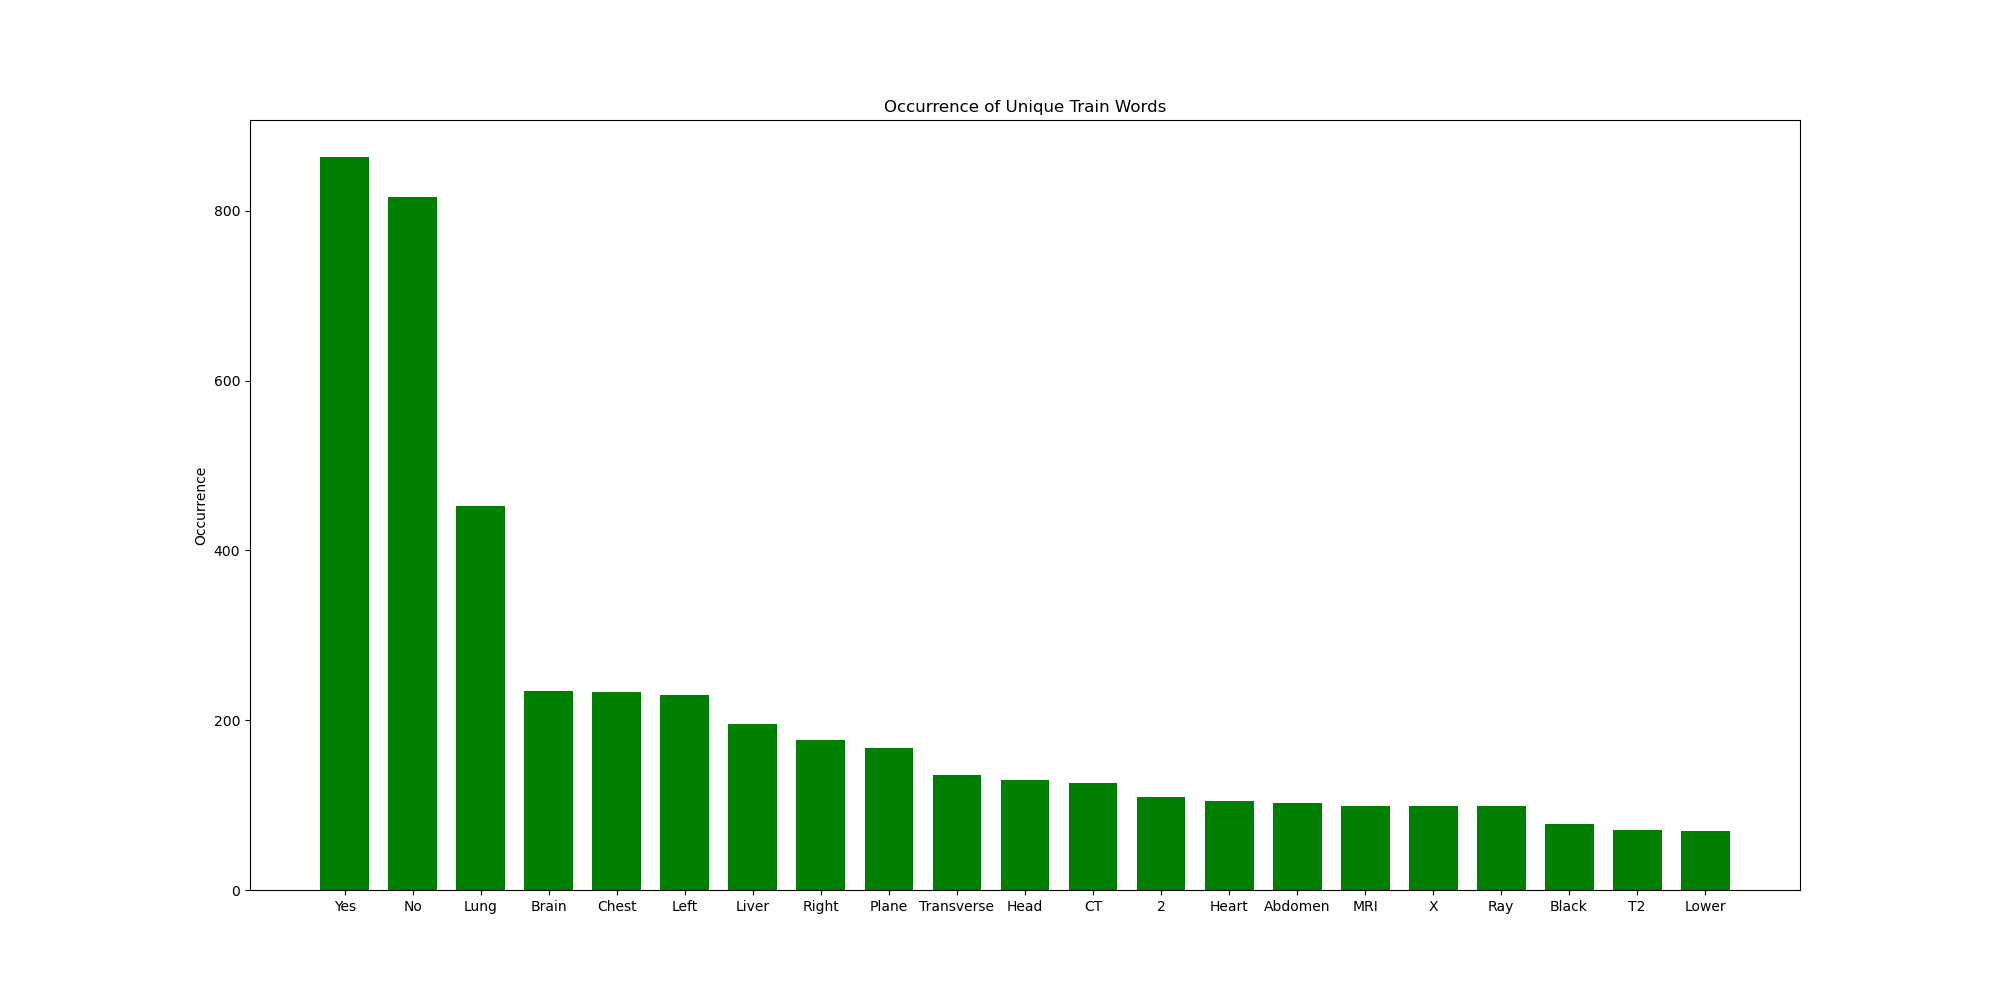
\includegraphics[width=15cm]{images/train_unique_words.png}
% \end{center}


%     \begin{center}
%          \hspace*{-1.5cm}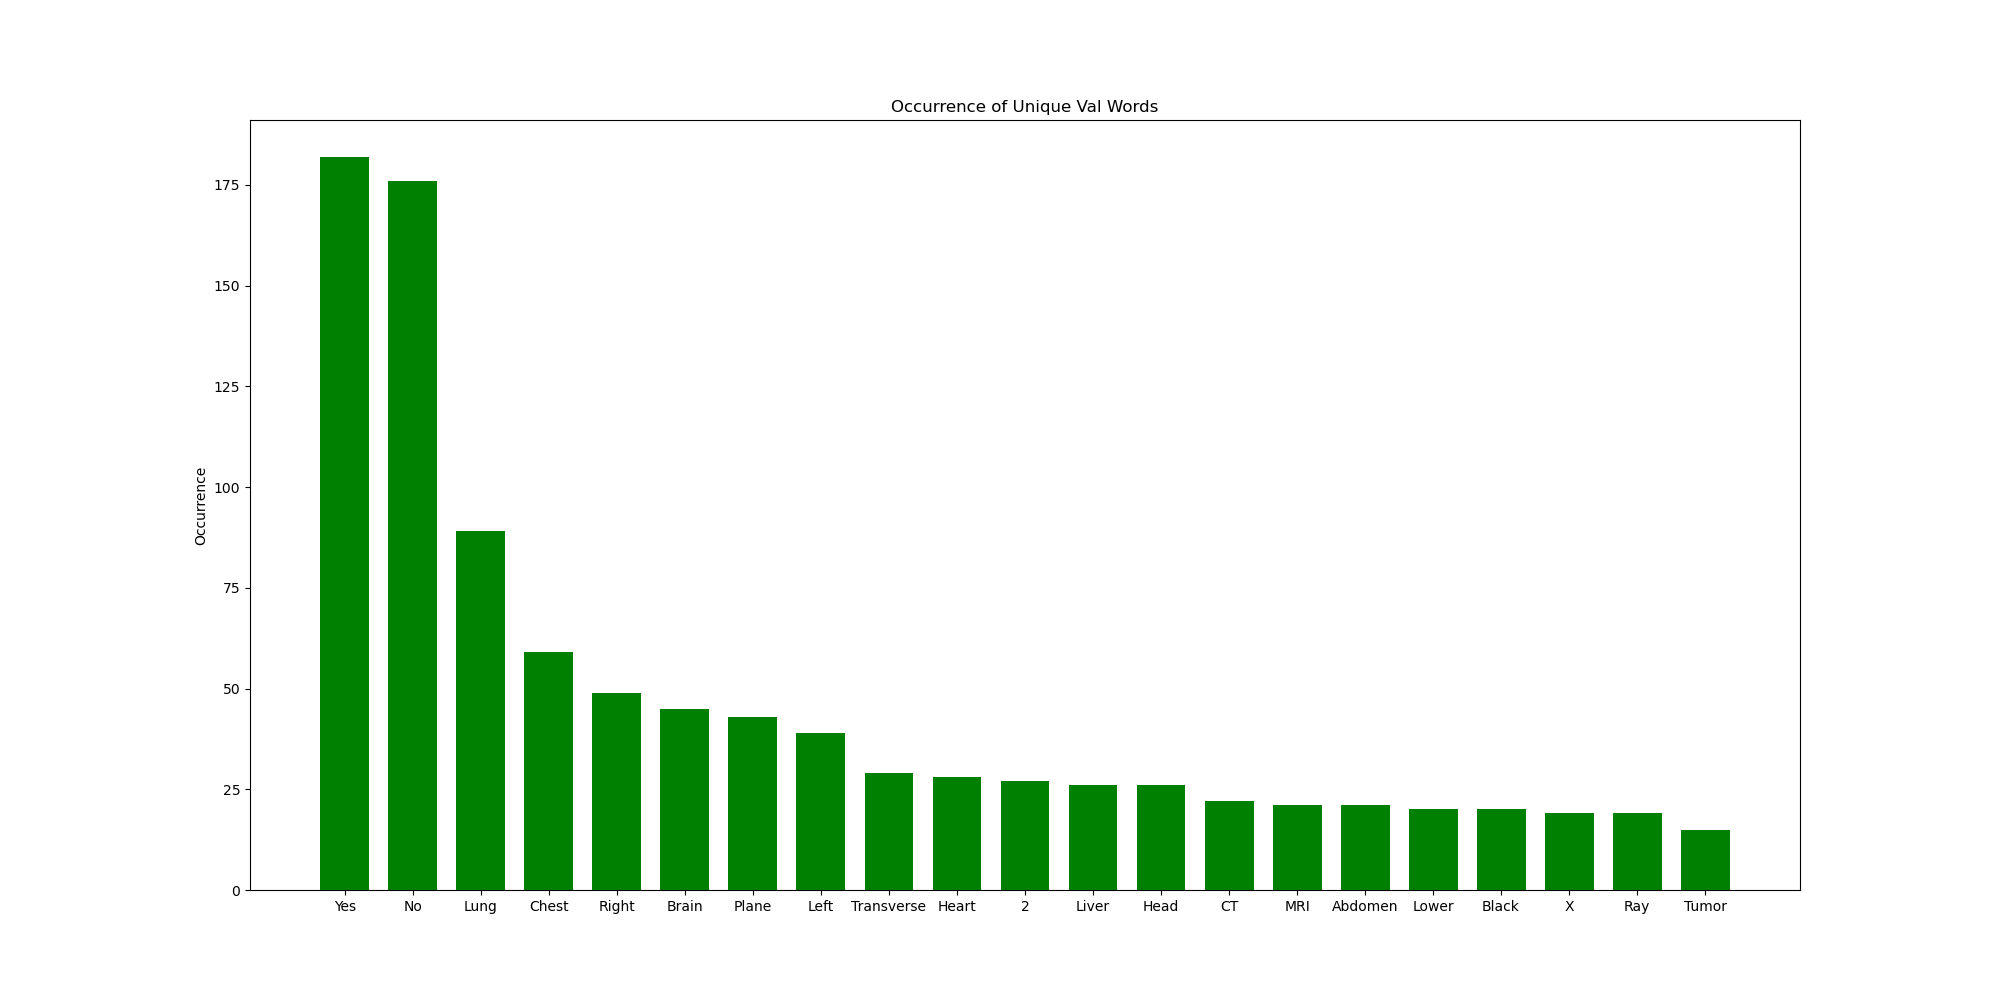
\includegraphics[width=15cm]{images/val_unique_words.png}
% \end{center}


%     \begin{center}
%          \hspace*{-1.5cm} 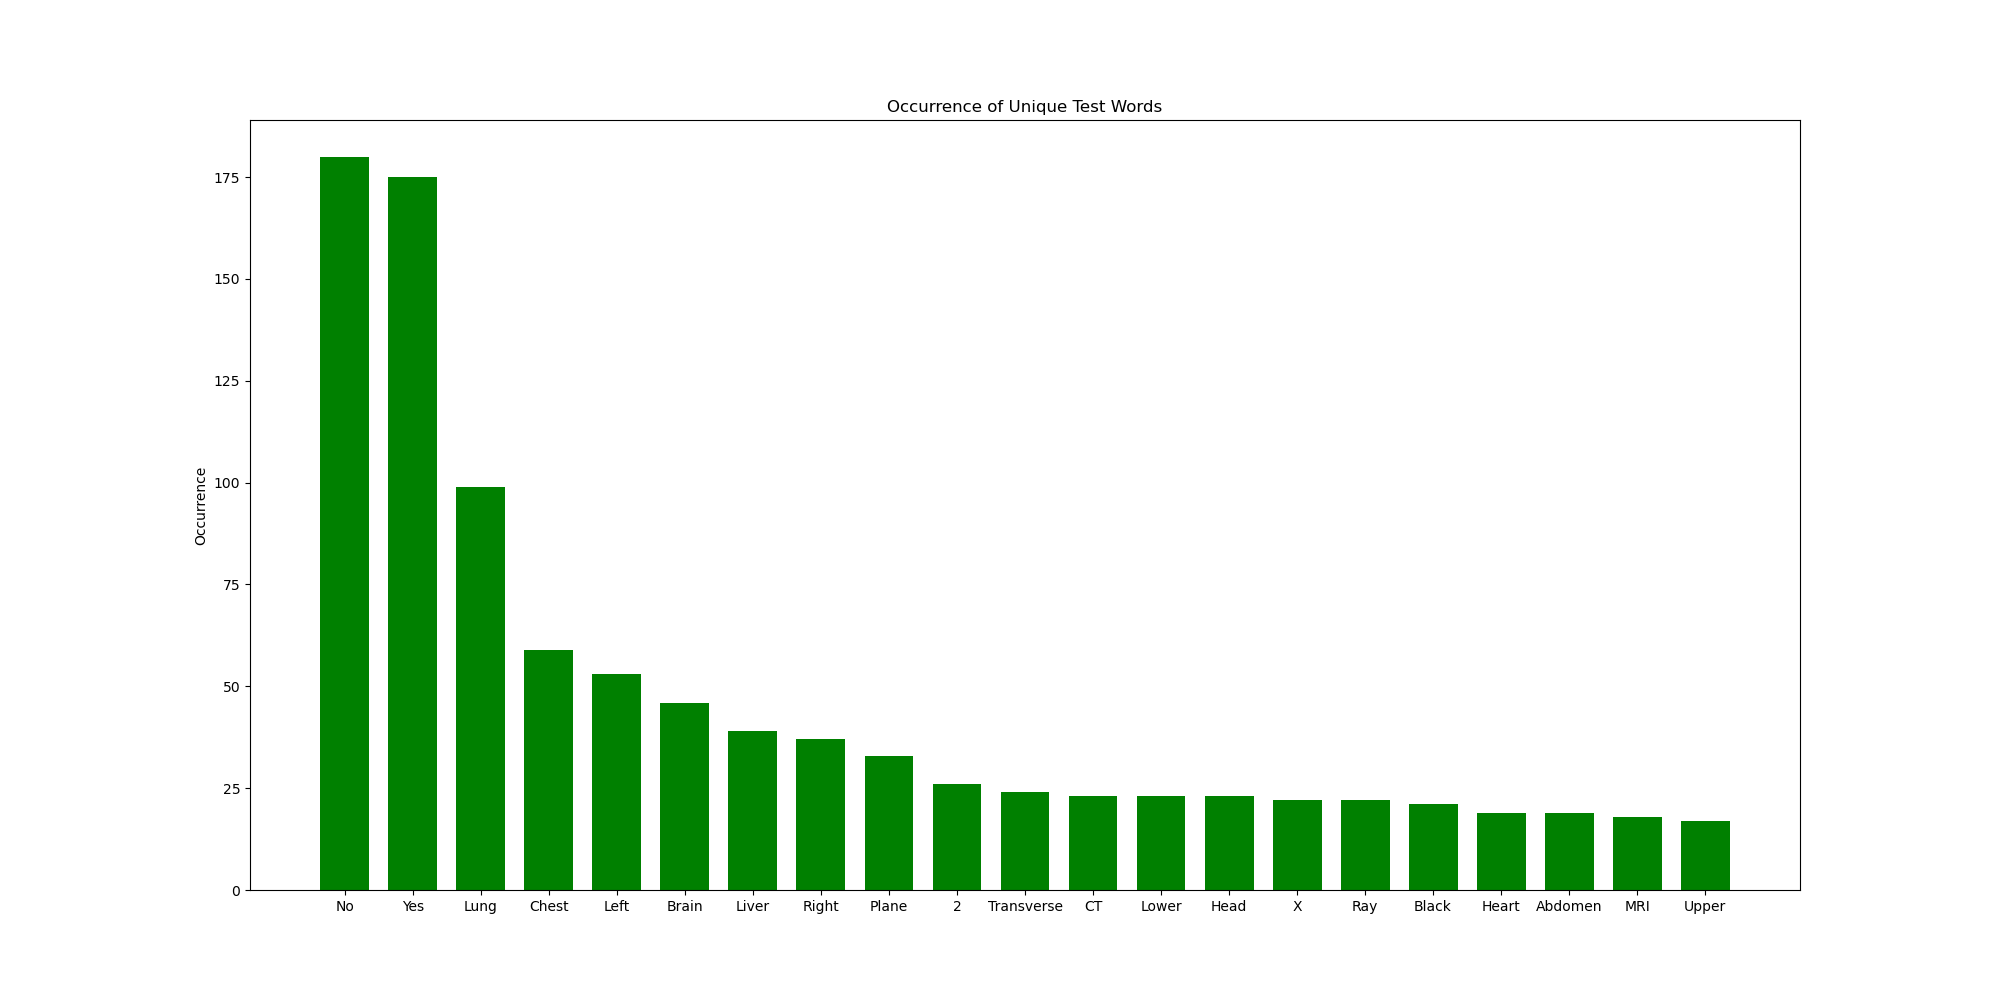
\includegraphics[width=15cm]{images/test_unique_words.png}
% \end{center}

% Note that due to the nature of the labels being comprised of single or multiple distinct words, it is not meaningful to assess measures such as the frequency of occurrence of label tokens, or identifying the most commonly appearing words.



 
	% \section{Layout}
	
	% 	The \textit{Adonis} template is based on the base \textit{article} template.
	% 	To use the template, you need to copy the \verb+adonis.cls+ class file to the same directory as your manuscript.
	% 	Then, specify the document class in the preamble:
		
	% 	\begin{verbatim}
	% 		\documentclass[twocolumn]{adonis}
	% 	\end{verbatim}
		
	% 	The paper dimensions are those of an A4 paper.
	% 	Many changes concern its layout, and most add white space.
	% 	The margins are wider, notably on the sides, but also at the top and bottom.
	% 	The extra space serves a dual purpose: an obvious aesthetic one, and a more functional one.
	% 	The wider margins afford margin notes more space, and thus gives them more prominence.
		
	% 	Unlike the \textit{article} template, \textit{Adonis} includes a header and a footer, albeit in small print.
	% 	The header shows the running author on the left and the running title on the right, while the footer shows the page number in the centre.
	% 	You can specify the running author and title as follows:
		
	% 	\begin{verbatim}
	% 		\runningauthor{Yours truly et al.}
	% 		\runningtitle{Short title}
	% 	\end{verbatim}
		
	% 	If you do not define them, the template uses the author and title fields instead.
	% 	\textit{Adonis} does not show the header and footer on the first page, which is already busy.
		
	% 	\subsection{Options}
		
	% 		The \textit{Adonis} template comes with optional directives to change how the manuscript looks.
	% 		By default, the template has one column and wide margins, but you can change both.
	% 		Remember that you can use multiple options, or none at all.
			
	% 		\subsubsection{Dark mode}
			
	% 			The dark mode sets a the page colour to a dark grey and the text to white to reduce eye strain during writing sessions.
	% 			To enable dark mode, pass the \texttt{dark} option to the \textit{Adonis} template:
				
	% 			\begin{verbatim}
	% 				\documentclass[dark]{adonis}
	% 			\end{verbatim}
			
	% 		\subsubsection{Legacy}
			
	% 			The legacy layout adds backwards compatibility for old packages.
	% 			Specifically, the legacy layout does not load the \texttt{notomath} package, which the template uses to render mathematical text.
	% 			Use the legacy layout on versions of TeX Live from before 2021, which do not include the package.
	% 			To enable the legacy layout, pass the \texttt{legacy} option to the \textit{Adonis} template:
				
	% 			\begin{verbatim}
	% 				\documentclass[legacy]{adonis}
	% 			\end{verbatim}
		
	% 		\subsubsection{Two columns}
			
	% 			The two-column layout gives the manuscript a conference paper-like look.
	% 			Since a two-column layout takes up more space, \textit{Adonis} reduces the margin sizes.
	% 			Part of the reclaimed margin size goes to the column separation to give the document a clean look and improve readability.
	% 			To enable the two-column layout, pass the \texttt{twocolumn} option to the \textit{Adonis} template:
			
	% 			\begin{verbatim}
	% 				\documentclass[twocolumn]{adonis}
	% 			\end{verbatim}
			
	% 		\subsubsection{Wide}
			
	% 			The default layout has wide margins, both to give the document a clean look and to reserve more space for margin notes.
	% 			If you require neither, you can reduce margin space and widen the text area by using the wide option:
			
	% 			\begin{verbatim}
	% 				\documentclass[wide]{adonis}
	% 			\end{verbatim}
	
	% 	\subsection{Front-matter}
		
	% 		\textit{Adonis} changes the \textit{article}'s front page to make a better first-impression.
	% 		The title is no longer centred nor justified, and in the two-column layout, it occupies only one column.
	% 		Moreover, to give the title more prominence, the template shrinks secondary information and moves some of it to the bottom of the page.
	% 		The template thus splits the front-matter into two parts, the main and secondary details.
			
	% 		\subsubsection{Main details}
			
	% 		The main details include three parts: the title, the author and the abstract.
	% 		To make the difference evident, the template gives the title a large font size and the author a smaller size, and italicizes the abstract.
	% 		A horizontal rule separates the abstract from the main content.
			
	% 		In the two-column layout, \textit{Adonis} also starts a new column after the abstract.
	% 		The white-space gives the template character and increases the separation between the abstract and the main text.
	% 		The title also appears slightly smaller in two-column layout, again due to the decreased space.
	% 		You can specify the title, author and abstract using dedicated commands:
			
	% 		\begin{verbatim}
	% 			\title{Your title}
	% 			\author{Yours truly}
	% 			\abstract{\lipsum[0]}
	% 		\end{verbatim}
			
	% 		\subsubsection{Secondary details}
			
	% 		The rest of the front-matter details, including the affiliations, the date of publication and the correspondence, appear at the bottom of the page in small type.\footnote{
	% 			To keep the template as simple as possible, \textit{Adonis} does not match the author with the affiliations.
	% 			In other words, you need to link the author with the affiliations manually, such as by adding superscript numbers next to your authors and next to their affiliations.
	% 		}
	% 		The secondary details are separated from the abstract and main text by a horizontal rule.
	% 		The template only renders the secondary details if you fill them in explicitly, so if you need a quick-start, you can leave them out altogether.
	% 		You can specify the secondary details using dedicated commands:
			
	% 		\begin{verbatim}
	% 			\affiliation{Affiliation}
	% 			\correspondence{youremail@tld.com}
	% 			\date{\today}
	% 		\end{verbatim}
		
	% \section{Typography}
	
	% 	The second major change concerns the typography.
	% 	\textit{Adonis} uses the Source font family to improve readability: Source Serif Pro for the main text, and Source Sans Pro for headings.
	% 	All paragraphs are justified to give the document a clean look.
		
	% 	\textit{Adonis} uses the same font size as in the base \textit{article} template: 10pt.
	% 	Differently from it, however, \textit{Adonis} uses a larger line-height: 1.4.
	% 	Apart from the normal size, the template also defines the \texttt{tiny}, \texttt{footnotesize}, \texttt{small}, \texttt{large} and \texttt{huge} sizes.
	% 	Font sizes larger than normal use a smaller line-height: about 1.2.
		
	% 	Moreover, \textit{Adonis} makes some subtler changes.
	% 	For example, the template uses the semi-bold font-weight in place of the actual bold-weight when using \texttt{\textbackslash{}textbf}, which looks more subtle next to the regular font-weight.
	% 	The template also uses the \texttt{microtype} package to enable protrusion and expansion; the former lets punctuation bleed slightly into the margins, and the latter uses varying font widths to make the word-spacing more even.
		
		% \subsection{Math}
		
		% 	The Source Pro family does not have support for mathematical text.
		% 	Instead, \textit{Adonis} uses the Noto Serif font to render mathematical text.
		% 	For example, the following equation represents the golden ratio $\phi$, on which I based the page margins.
		% 	The font has a thickness much closer to Source Serif's than the default font.
		
		% 	\begin{equation}
		% 		\phi = \frac{1 + \sqrt{5}}{2}
		% 	\end{equation}
		
		% 	Note that the \texttt{notomath} package is only available from TeX Live 2021 onward.
		% 	To use the template on earlier versions, pass the \texttt{legacy} option to the document class:
			
		% 	\begin{verbatim}
		% 		\documentclass[legacy]{adonis}
		% 	\end{verbatim}

		% \subsection{Headings}
		
		% 	Unlike the rest of the text, headings use the Source Sans Pro family.
		% 	All headings have the same size as the text, but they have a semi-bold font-weight and a small-caps shape.
		% 	The different font serves to draw attention to headings, and thus make the manuscript easier to navigate.
		% 	\textit{Adonis} supports three heading levels.
		
		% 	\subsubsection{Section}
			
		% 		The section is the highest level in manuscripts.
		% 		Therefore \textit{Adonis} adds a hefty margin before them, such that sections leap out when scrolling.
			
			
			
			
	% \section{Other elements}
	
	% 	\begin{table*}[t!]
	% 		\begin{tabularx}{\linewidth}{ l l X }
	% 			\textbf{Version} & \textbf{Date} & \textbf{Changelog} \\ \hline
	% 			0.1 & April 16, 2023 & Initial release \\
	% 			0.2 & May 12, 2023   & Improved text readability, new math font and \texttt{legacy} option, dark mode, and miscellaneous layout changes \\
	% 		\end{tabularx}
	% 		\caption{The template's version history.}
	% 		\label{"Table: version history"}
	% 	\end{table*}
	
	% 	In addition to the layout and typography, \textit{Adonis} also makes slight changes to other common \LaTeX{} elements.
	% 	The template gives table cells more padding and rows more space, as shown in Table~\ref{"Table: version history"}.

	% 	Margin notes also use a smaller font size such that they are not too prominent.
	
	
	\begin{thebibliography}{5}
		\bibitem{slake}
		SLAKE: A Semantically-Labeled Knowledge-Enhanced Dataset for Medical Visual Question Answering. Bo Liu, Li-Ming Zhan, Li Xu, Lin Ma, Yan Yang, Xiao-Ming Wu (2021). \url{https://arxiv.org/abs/2102.09542}

		\bibitem{FSVQA}
		The Color of the Cat is Gray: 1 Million Full-Sentences Visual Question Answering (FSVQA). Andrew Shin, Yoshitaka Ushiku, Tatsuya Harada (2016). \url{https://doi.org/10.48550/arXiv.1609.06657}
	

		\bibitem{genvqa}
		Generate Answer to Visual Questions with Pre-trained
Vision-and-Language Embeddings. Hadi Sheikhi, Maryam Hashemi, Sauleh Eetemad (2022). \url{https://www.winlp.org/wpcontent/uploads/2022/11/73_Paper.pdf}
	\end{thebibliography}
	
\end{document}